\documentclass[runningheads]{llncs}
\usepackage{graphicx}
\usepackage{tabularx}
\usepackage{amsmath}
\usepackage{multirow}
\newcommand{\code}[1]{\texttt{#1}}
\usepackage{xcolor}
\usepackage{fancyvrb}
\usepackage{listings}
\lstloadlanguages{Python}
\lstset{
  language=Python,
  basicstyle=\scriptsize\sffamily,
  numberstyle=\color{gray},
  stringstyle=\color[HTML]{933797},
  commentstyle=\color[HTML]{228B22}\sffamily,
  emph={[2]from,import,pass,return}, emphstyle={[2]\color[HTML]{DD52F0}},
  emph={[3]range}, emphstyle={[3]\color[HTML]{D17032}},
  emph={[4]for,in,def}, emphstyle={[4]\color{blue}},
  showstringspaces=false,
  breaklines=true,
  prebreak=\mbox{{\color{gray}\tiny$\searrow$}},
  numbers=left,
  xleftmargin=15pt
}

%%%%% START DOCUMENT %%%%%
\begin{document}

\title{COMP 472 Project 2 \\ Naive Bayes Classifier}

\author{Matteo Esposito\inst{1} \and
Matthew Liu\inst{2} \and
Kabir Soni\inst{3}}

\authorrunning{M. Esposito et al.}

\institute{40024121 \email{matteoesposito97@gmail.com} \and
40029238 \email{matthew.jx.liu@gmail.com} \and
40033019 \email{kabirsoni524@gmail.com}}

\maketitle   

\section{Introduction \& Technical Details}

This project was developed using python 3.7.4 64-bit.

\subsection{Files}

The file structure of our project is as follows:

\begin{table}
    \centering
    \caption{Files in project 1}\label{tab0}
    \begin{tabularx}{\textwidth}{|l|l|X|}
        \hline
        \textbf{Directory} & \textbf{Filename} & \textbf{Usage} \\ \hline
        \verb|out/| & * & Trace and evaluation files for each run. \\ \hline
        \verb|out_BYOM/| & * & Trace and evaluation files for each BYOM run. \\ \hline
        \verb|src/| & \verb|utils.py| & Helper functions for I/O and input parsing. \\ \hline
                    & \verb|NBClassifier.py| & Naive Bayes Classifier class. A collection of methods used to implement Naive Bayes Classification. \\ \hline
                    & \verb|Ngram.py| & Ngram class, used in all classifications. \\ \hline
                    & \verb|BYOM.py| & Personalized model class. \\ \hline
                    & \verb|main.py| & Reading training set, training classifier, predicting languages on test set and writing out results. \\ \hline
    \end{tabularx}
\end{table}

\subsection{Packages}

We used a total of 7 packages in our project, 5 existing, along with our 2 internal packages (board and node). 

\begin{enumerate}
    \item Existing 
    \begin{itemize}
        \item \verb|shutil| and \verb|os|: Folder and file management in the creation and deletion of output folders for our search and solution files. 
        \item \verb|math|: Calculating log base 10 probabilities as part of the score function of each tweet.
        \item \verb|copy|: Used to create deep copies in the initialization of ngrams in the NBClassifier class.
        \item \verb|decimal.Decimal|: Used to format the probability output for the trace file.
        \item \verb|string|: Used to populate vocabulary 1 and 2 with ascii characters.
    \end{itemize}
    \item Internal
    \begin{itemize}
        \item \verb|NBClassifier|: Class that is used to represent the classifier, which takes a vocabulary selection, ngram size, delta/smoothing value and train/test file links.
        \item \verb|Ngram|: Class used to represent the Ngram used in the NBClassifier class. 
    \end{itemize}
\end{enumerate}

\subsection{NBClassifier and Ngram Classes}

The \textbf{Ngram} class will be used in the NBClassifier class. It allows for a concise way to store a language, count/frequency table, probability table and language probability. This class stores the probability calculation, smoothing and language probability methods which are called in the train method of NBClassifier.

\medskip

The \textbf{NBClassifier} class will have as main attributes a language, count table, probability table and size $(n)$, which will all be stored in a size-$n$ Ngram. It will also hold a language probability. It is from the NBClassifier object in \code{main.py} that we will call the train and predict methods.

\medskip

\underline{Note on vocabulary creation:} Vocabularies 0 and 1 are generated by combining ascii character sets from the \code{string} library. Vocabulary 3 is created by...
\textcolor{red}{Matt add something here that talks about the creation of vocab2 for Ngrams}

\newpage

\section{Dataset Impact \& Analysis}

In our exploratory data analysis we assess 2 characteristics of the test sets, namely tweet length and language frequency.

\subsection{Tweet Length}

Rounding down all tweets with length larger than 150 charaters down to 150 (as they make up less than 0.5\% of the observations), we get the following capped tweet length distribution curves for the provided and demo test sets of tweets.

\begin{figure}
    \begin{center}
        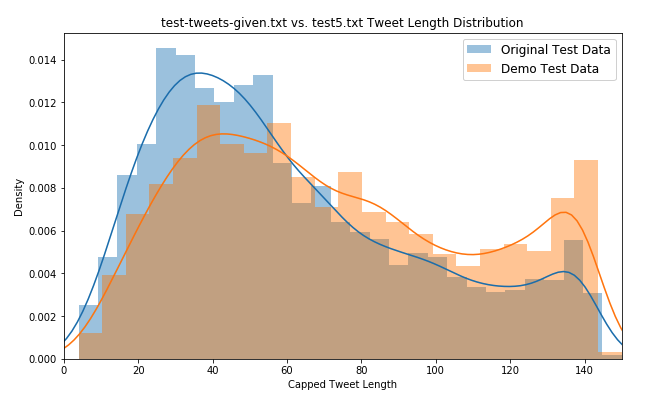
\includegraphics[width=12.5cm]{images/tlendist.png}
    \end{center}
\end{figure}

The main observation we can notice from the overlayed distribution plots is that the demo test set contains a greater proportion of large tweets (tweets with length over $\sim 70$ characters). The effect this could have on the accuracy of our classifications is that we are introducing a larger amount of unigrams, bigrams and trigrams from the tweet being assessed by the classifier and therefore introducing the potential for a greater amount of incorrectly labelled character patterns.

\subsection{Language Frequency}

Generating a frequency table of the languages in the provided test dataset we observe the following:

\begin{verbatim}
orig_test.lang.value_counts()

    es    3926
    pt    2020
    en     505
    eu     376
    ca      75
    gl       1

\end{verbatim}

We notice that there is a single observation in the 'gl' class. This will have an effect on our precision, recall and f1 values. In the case where we do not correctly classify that observation into the 'g1' class, our true positive value for the gl class will be 0, making precision and recall also 0 and yielding an f1 value of $0/0$ (which we set to 0 in this case).

\medskip

Generating a frequency table of the languages in the demo test dataset we observe the following:

\begin{verbatim}
demo_test.lang.value_counts()

    es    4572
    ca    1387
    gl     504
    en     483
    pt      96

\end{verbatim}

We notice that there are no observation in the 'eu' class. Every classification of a test tweet into the 'eu' class will result in a direct increase in the number of false positives, affecting our validation metrics negatively (decreasing precision and f1).

\section{Our Model (BYOM)}

\textcolor{red}{Kabir}

\section{Result \& Experiment Analysis}

\textcolor{red}{Check in appendix for all necessary confusion matrices}

\section{Team Responsibilities}

The breakdown of tasks were as follows:

\begin{enumerate}
    \item Matteo Esposito
    \begin{itemize}
        \item Project structure
        \item NBClassifier \& Ngram class
        \item utility functions \code{utils.py}
    \end{itemize}
    \item Matthew Liu
    \begin{itemize}
        \item NBClassifier \& Ngram class
        \item utility functions \code{utils.py}
    \end{itemize}
    \item Kabir Soni
    \begin{itemize}
        \item Personalized model (BYOM)
    \end{itemize}
\end{enumerate}

\begin{thebibliography}{8}
    
\bibitem{ref_2}
S.J. Russel, P. Norvig: Artificial Intelligence: A Modern Approach. 3rd edn. Pearson, Harlow (1994)

\end{thebibliography}

\section{Appendices}
\subsection{Appendix A - Confusion Matrices (Given Test Dataset \code{test-tweets-given.txt})}

\begin{table}
	\centering
	\caption{Cross tabulation of predictions, $V=0, n=1, \delta=0$}
	\begin{tabular}{|c|c|c|c|c|c|c|c|} \hline
		& & \multicolumn{6}{c|}{Predicted} \\ \hline
		& &  ca &   en &    es &   eu &  gl &   pt \\ \hline
		\multirow{6}{*}{Actual} & ca   &  24 &    3 &    44 &    1 &   1 &    2 \\
		& en   &   7 &  287 &   205 &   11 &   0 &    6 \\
		& es   &  44 &  140 &  3635 &   63 &   3 &   88 \\
		& eu   &   3 &   16 &   107 &  253 &   0 &    1 \\
		& gl   &   0 &    0 &     1 &    0 &   0 &    0 \\
		& pt   &  16 &   62 &  1365 &   11 &   1 &  600 \\ \hline
	\end{tabular}
\end{table}

\begin{table}
	\centering
	\caption{Cross tabulation of predictions, $V=1, n=2, \delta=0.5$}
	\begin{tabular}{|c|c|c|c|c|c|c|c|} \hline
		& & \multicolumn{6}{c|}{Predicted} \\ \hline
		& &   ca &   en &    es &   eu &  gl &    pt \\ \hline
		\multirow{6}{*}{Actual} & ca   &   59 &    1 &    14 &    0 &   0 &     1 \\
		& en   &    8 &  443 &    50 &    7 &   0 &     8 \\
		& es   &  110 &   66 &  3584 &   84 &  41 &    88 \\
		& eu   &    5 &    6 &    41 &  323 &   0 &     5 \\
		& gl   &    0 &    0 &     0 &    0 &   0 &     1 \\
		& pt   &   61 &   23 &   397 &    8 &  38 &  1528 \\ \hline
	\end{tabular}
\end{table}

\begin{table}
	\centering
	\caption{Cross tabulation of predictions, $V=1, n=3, \delta=1$}
	\begin{tabular}{|c|c|c|c|c|c|c|c|} \hline
		& & \multicolumn{6}{c|}{Predicted} \\ \hline
		& &  ca &   en &    es &   eu &  gl &    pt \\ \hline
		\multirow{6}{*}{Actual} & ca   &  53 &    1 &    21 &    0 &   0 &     0 \\
		& en   &   4 &  386 &   121 &    1 &   0 &     4 \\
		& es   &  10 &   15 &  3918 &    6 &   1 &    23 \\
		& eu   &   5 &    4 &   140 &  230 &   0 &     1 \\
		& gl   &   0 &    0 &     1 &    0 &   0 &     0 \\
		& pt   &  16 &    8 &   480 &    0 &   1 &  1550 \\ \hline
	\end{tabular}
\end{table}


\begin{table}
	\centering
	\caption{Cross tabulation of predictions, $V=2, n=2, \delta=0.3$}
	\begin{tabular}{|c|c|c|c|c|c|c|c|} \hline
		& & \multicolumn{6}{c|}{Predicted} \\ \hline
		& &  ca &   en &    es &   eu &  gl &    pt \\ \hline
		\multirow{6}{*}{Actual} & ca   &  62 &    1 &    12 &    0 &   0 &     0 \\
		& en   &   9 &  438 &    60 &    7 &   0 &     2 \\
		& es   &  70 &   55 &  3721 &   57 &  11 &    59 \\
		& eu   &   4 &    8 &    51 &  311 &   0 &     6 \\
		& gl   &   0 &    0 &     0 &    0 &   0 &     1 \\
		& pt   &  47 &   20 &   340 &    6 &  14 &  1628 \\ \hline
	\end{tabular}
\end{table}

\begin{table}
	\centering
	\caption{Cross tabulation of predictions (BYOM), $V=1, n=2, \delta=0.5$}
	\begin{tabular}{|c|c|c|c|c|c|c|c|} \hline
		& & \multicolumn{6}{c|}{Predicted} \\ \hline
		& &  ca &   en &    es &   eu &  gl &    pt \\ \hline
		\multirow{6}{*}{Actual} & ca   &  51 &    1 &    23 &    0 &   0 &     0 \\
		& en   &   3 &  406 &   102 &    2 &   0 &     3 \\
		& es   &  11 &   16 &  3914 &    7 &   0 &    25 \\
		& eu   &   2 &    4 &   109 &  264 &   0 &     1 \\
		& gl   &   0 &    0 &     1 &    0 &   0 &     0 \\
		& pt   &  17 &    9 &   412 &    0 &   2 &  1615 \\ \hline
	\end{tabular}
\end{table}

\newpage

\subsection{Appendix B - Confusion Matrices (Demo Dataset \code{test5.txt})}

\begin{table}
	\centering
	\caption{Cross tabulation of predictions, $V=0, n=1, \delta=0$}
	\begin{tabular}{|c|c|c|c|c|c|c|c|} \hline
        & & \multicolumn{6}{c|}{Predicted} \\ \hline
		& &    ca &   en &    es &  eu &   gl &   pt \\ \hline
		\multirow{6}{*}{Actual} & ca   &  418 &   52 &   868 &   5 &   5 &   43 \\
		& en   &    7 &  299 &   171 &   2 &   0 &    4 \\
		& es   &   51 &  164 &  4217 &  20 &   5 &  132 \\
		& gl   &    7 &    8 &   441 &   1 &   8 &   41 \\
		& pt   &    0 &    5 &    61 &  10 &   0 &   20 \\ \hline
		\end{tabular}

\end{table}
\begin{table}
	\centering
	\caption{Cross tabulation of predictions, $V=1, n=2, \delta=0.5$}
	\begin{tabular}{|c|c|c|c|c|c|c|c|} \hline
	    & & \multicolumn{6}{c|}{Predicted} \\ \hline
		& &    ca &   en &    es &  eu &   gl &   pt \\ \hline
		\multirow{6}{*}{Actual} & ca   &  1064 &   23 &   256 &   7 &    9 &   32 \\
		& en   &    34 &  380 &    59 &   2 &    0 &    8 \\
		& es   &   150 &   99 &  4072 &  32 &  107 &  129 \\
		& gl   &    19 &    9 &   266 &   4 &  122 &   86 \\
		& pt   &     4 &    1 &    19 &   1 &    2 &   69 \\ \hline
	\end{tabular}
\end{table}

\begin{table}
	\centering
	\caption{Cross tabulation of predictions, $V=1, n=3, \delta=1$}
	\begin{tabular}{|c|c|c|c|c|c|c|c|} \hline
	    & & \multicolumn{6}{c|}{Predicted} \\ \hline
		& &    ca &   en &    es &  eu &  gl &  pt \\ \hline
		\multirow{6}{*}{Actual} & ca   &  1041 &    4 &   338 &   0 &   0 &   8 \\
		& en   &    21 &  329 &   131 &   0 &   0 &   2 \\
		& es   &    20 &   40 &  4480 &   1 &   6 &  42 \\
		& gl   &     3 &    1 &   452 &   0 &  19 &  31 \\
		& pt   &     2 &    0 &    29 &   0 &   0 &  65 \\ \hline
	\end{tabular}
\end{table}

\newpage

\begin{table}
	\centering
	\caption{Cross tabulation of predictions, $V=2, n=2, \delta=0.3$}
	\begin{tabular}{|c|c|c|c|c|c|c|c|} \hline
	    & & \multicolumn{6}{c|}{Predicted} \\ \hline
		& &    ca &   en &    es &  eu &   gl &  pt \\ \hline
		\multirow{6}{*}{Actual} & ca   &  1107 &   18 &   239 &   7 &    2 &  18 \\
		& en   &    29 &  374 &    72 &   1 &    0 &   7 \\
		& es   &   114 &   84 &  4227 &  20 &   52 &  92 \\
		& gl   &    11 &    6 &   326 &   1 &  106 &  56 \\
		& pt   &     1 &    0 &    18 &   1 &    0 &  76 \\ \hline
	\end{tabular}
\end{table}

\begin{table}
	\centering
	\caption{Cross tabulation of predictions (BYOM), $V=1, n=2, \delta=0.5$}
		\begin{tabular}{|c|c|c|c|c|c|c|c|} \hline
		& & \multicolumn{6}{c|}{Predicted} \\ \hline
		& &  ca &   en &    es &  eu &  gl &  pt \\ \hline
		\multirow{6}{*}{Actual} & ca   &  1071 &    7 &   305 &   0 &   0 &   8 \\
		& en   &    22 &  342 &   116 &   0 &   0 &   3 \\
		& es   &    19 &   44 &  4465 &   1 &  13 &  47 \\
		& gl   &     4 &    2 &   415 &   0 &  42 &  43 \\
		& pt   &     2 &    0 &    25 &   0 &   0 &  69 \\ \hline
    \end{tabular}
\end{table}

\subsection{Appendix C - Miscellaneous Code}

\subsubsection{Confusion Matrix}

\begin{lstlisting}[breaklines]
import pandas as pd

# Go through all the trace files generated during the demo.
for file in ['trace_0_1_0.txt', 'trace_1_2_0.5.txt', 'trace_1_3_1.txt', 'trace_2_2_0.3.txt', 'trace_1_BYOM_0.5.txt']:
    df = pd.read_csv(f'total_out/{file}', delimiter="  ", names=('id','lang','prob','pred_lang','res'))
    print(pd.crosstab(df['lang'], df['pred_lang']).to_latex())
\end{lstlisting}

\subsubsection{Distribution Plot}


\begin{lstlisting}[breaklines, language=Python]
import seaborn as sns
import pandas as pd
import matplotlib.pyplot as plt

orig_test = pd.read_csv(f'input/test-tweets-given.txt', delimiter="\t", names=('id','user','lang','tweet'))
demo_test = pd.read_csv(f'input/test5.txt', delimiter="\t", names=('id','user','lang','tweet'))

fig, ax = plt.subplots(figsize=(10,6))

# Cap data at tweet length of 150 and create individual plots.
orig_test['tlen'] = orig_test['tweet'].apply(len)
orig_test['tlen_capped'] = np.where(orig_test['tlen'] > 150, 150, orig_test['tlen'])
sns.distplot(orig_test.tlen_capped, ax=ax, label="Original Test Data")

demo_test['tlen'] = demo_test['tweet'].apply(len)
demo_test['tlen_capped'] = np.where(demo_test['tlen'] > 150, 150, demo_test['tlen'])
sns.distplot(demo_test.tlen_capped, ax=ax, label="Demo Test Data")

# Settings
plt.xlim(0, 150)
plt.title('test-tweets-given.txt vs. test5.txt Tweet Length Distribution')
plt.xlabel('Capped Tweet Length')
plt.legend(prop={'size': 12})
plt.ylabel('Density')
\end{lstlisting}

\end{document}

